% REMEMBER TO SET LANGUAGE!
\documentclass[a4paper,12pt,norsk]{article}
\usepackage[utf8]{inputenc}
% Standard stuff
\usepackage{amsmath,amsthm, amssymb,graphicx,varioref,verbatim,amsfonts,geometry,esint,url}
% colors in text
\usepackage[usenames,dvipsnames,svgnames,table]{xcolor}
% Hyper refs
\usepackage[colorlinks]{hyperref}
\usepackage{float}
\usepackage{wrapfig}
\usepackage{multicol}

\usepackage[export]{adjustbox}

\usepackage{subfig}

% Document formatting
\setlength{\parindent}{0mm}
\setlength{\parskip}{1.5mm}

%Color scheme for listings
\usepackage{textcomp}
\definecolor{listinggray}{gray}{0.9}
\definecolor{lbcolor}{rgb}{0.9,0.9,0.9}

\usepackage{listings}
\lstset{
	backgroundcolor=\color{lbcolor},
	tabsize=4,
	rulecolor=,
	language=python,
        basicstyle=\scriptsize,
        upquote=true,
        aboveskip={1.5\baselineskip},
        columns=fixed,
	numbers=left,
        showstringspaces=false,
        extendedchars=true,
        breaklines=true,
        prebreak = \raisebox{0ex}[0ex][0ex]{\ensuremath{\hookleftarrow}},
        frame=single,
        showtabs=false,
        showspaces=false,
        showstringspaces=false,
        identifierstyle=\ttfamily,
        keywordstyle=\color[rgb]{0,0,1},
        commentstyle=\color[rgb]{0.133,0.545,0.133},
        stringstyle=\color[rgb]{0.627,0.126,0.941}
        }
        
\DeclareMathOperator{\dist}{dist}
\newcommand{\distx}{\dist x}
        
\newcounter{subproject}
\renewcommand{\thesubproject}{\alph{subproject}}
\newenvironment{subproj}{
\begin{description}
\item[\refstepcounter{subproject}(\thesubproject)]
}{\end{description}}

%Lettering instead of numbering in different layers
%\renewcommand{\labelenumi}{\alph{enumi}}
%\renewcommand{\thesubsection}{\alph{subsection}}

%opening

\title{Fys4150 Project 1}
\author{Aksel Graneng}

\begin{document}
\maketitle

\abstract{This paper looks at solving differential equations as sets of linear equations, and concludes with the importance of writing non-generalized code for matrix operations.}

\section{Introduction}
	In this project, we will be solving a differential equation as a set of linear equations. This will be done using algorithms of varying generalization in python.\\
	We will look at just how row reduction can solve a differential equation, as well as the efficiency in different row reduction methods.

\section{Theory}

\subsection{Vectorized second derivative}

	If we have a 1d data-set on the form:
	$$\vec{V(x)} = [v_0,\ v_1,\ \cdots,\ v_{n-1},\ v_{n},\ v_{n-1},\ \cdots] $$\\
	Then we can write the second derivative of the data-set as:
	$$f_n = -\frac{v_{n+1} + v_{n-1} - 2v_n}{\Delta x^2} $$\\
	Where $\Delta x$ is the change in variable we are derivating based on; usually time.\\
	\\
	Rather than calculating the second derivatives of this data-set individually, we can instead calculate them all at the same time using linear algebra.\\
	This can be done by finding a matrix $A$ such that
	$$A\vec{V} = \vec{f} $$\\
	Where:
	\begin{gather*}
	\vec{f} = \left[
	\begin{array}{c}
	2v_i - v_2\\
	-v_1 + 2v_2 - v_3\\
	\vdots\\
	-v_{n-1} + 2v_n -v_{n+1}\\
	-v_n + 2v_{n+1} - v_{n+2}\\
	\vdots
	\end{array}
	\right]
	\end{gather*}
	As multiplying $\vec{f}$ with $\frac{1}{\Delta x^2}$ would give us an array containing all the second derivatives. We can see that $\textbf{A}$ must be:
	\begin{gather*}
	\textbf{A} = \left[
	\begin{array}{ccccc}
	2 & -1 & 0 & 0 & \cdots\\
	-1 & 2 & -1 & 0 & \cdots\\
	0 & -1 & 2 & -1 & \cdots\\
	\vdots & 0 & -1 & 2 & -1
	\end{array}
	\right]
	\end{gather*}

	This matrix can then be used to put up a set of linear equations:
	$$\textbf{A}\textbf{v} = \textbf{f} $$\\
	Where $\textbf{v}$ contains solutions to the differential equation:
	$$-u''(x) = f(x) $$
	
\section{Method}
	\subsection{General linear equation solver}
	The first thing our program does is solve a set of general linear equations on the form $\textbf{A}\textbf{v} = \textbf{f}$. This is done by putting the matrix $\textbf{M}$ on row reduced echeleon form:
	\begin{gather*}
	\textbf{M} =  \left[
	\begin{array}{cccccc}
	b_1 & c_1 & 0 & 0 & \cdots f_1\\
	a_2 & b_2 & c_2 & 0 & \cdots f_2\\
	0 & a_3 & b_3 & b_3 & \cdots f_3\\
	\vdots & 0 & a_4 & b_4 & \cdots f_4
	\end{array}
	\right]
	\end{gather*}

	Where $\textbf{M}$ is a $n \times (n+1)$ matrix. This is generally quite simple to solve using forward and backward substitution, but when $n$ becomes very large (in my experience, larger than $10^5$) we get problems with memory as well as computation time, as the most simple row reduction algorithm has $2(n+1)n^2$ FLOPS.\\
	To avoid this problem, we use the fact that most of the elements in the matrix is zero. In fact, there are at most 4 elements in each row that isnt zero. By removing every element that is zero from the matrix (except one in for the first and last line), we get:

\begin{gather*}
	\textbf{M}^* = \left[
	\begin{array}{cccc}
	b_1 & c_1 & 0 & f_1\\
	a_2 & b_2 & c_2 & f_2\\
	\vdots & \vdots & \vdots & \vdots\\
	0 & a_n & b_n & f_n
	\end{array}
	\right]
	\end{gather*}

	So now we have a $n \times 4$ matrix which contains all the information we need.\\
	\\
	We now use forward substitution on $\textbf{M}^*$ just like we would on $\textbf{M}$, except this time we "roll" the next row every time we subtract, so that $b_i$ is subtracted from $a_{i+1}$ and $c_i$ is subtracted from $b_{i+1}$. At the same time, we are careful to subtract $f_i$ from $f_{i+1}$. This means that index notation must be used, rather than numpy.roll.\\
	This is done in a loop that has $n$ iterations. First it does 3 operations, one on each element in the row except for the first (which is zero), along with a division, to normalize it. Then it does 3 subtraction and multiplication operations on the next row.\\
	\\
	Next is backwards substitution. Again we use a loop with n iterations. Here we only do 2 subtractions and multiplications, on the last and second last element of each row.\\
	All in all, this sums up to $14n$ FLOPS.\\
	\\
	After it was done, the general linear equation solver was tested on:
	\begin{gather*}
		u''(x) = f(x)\\
		\\
		f(x) = 100e^{-10x}
	\end{gather*}
	Which has a closed-form solution:
	$$u(x) = 1 - (1 - e^{-10})x - e^{-10x} $$

	\subsection{Specific linear equation solver}
	The matrix we are working with in this project is very simple. All values of $a$, all values of $b$ and all values of $c$ are equal. That is to say: 
	$$\text{for any }i \wedge j \in [1,\ n],\ a_i = a_j,\ b_i = b_j,\ c_i = c_j$$\\
	This means that we are practically doing the same operations n times when we are row reducing our matrix. Rather than doing this, we can limit our algorithm to only operate on our values for $f$, as these are unknown. We simply need to look at what the row reduction algorithm does to the matrix to see what it does to $f$, and then skip right to that part when calculating it numerically.\\
	\\
	Studying the forward substitution, we see, starting with $n = 2$:
	$$f_n^* = \frac{n}{n+1}(f_n - f_{n-1}^*) $$\\
	Thus, the n'th row ends up as (excluding all the zeros):
	$$[0,\ 1,\ -\frac{n}{n+1},\ f_n^*] $$\\
	The very last row ends up as (with $n = \text{size of $f$}$):
	$$[0,\ 0,\ 1,\ -(f_{-1}-f^*_{-2})\frac{n}{n+1}] $$\\
	The first value of $f$ (n = 1) ends up as:
	$$f_1^* = \frac{1}{2}f_1 $$\\
	\\
	And then we look at backwards substitution. We can see that we subtract:
	$$\frac{n-i}{n-i-1}f^{**}_{-(i-1)} $$\\
	from $f^*_{-i}$ to find our final value $f_{-i}^{**}$\\
	The process of forward substitution ends with the last line being:
	$$f^*_1 = f^*_1 + 2f_2^{**} $$\\

	The specified algorithm for solving the linear equations is a lot more efficient than the general one. Assuming we have already calculated the required numbers used in finding $f$, the forwards and backwards substitutions each require 2 operations, resulting in a total of $4n$ FLOPS.

	\subsection{LU Decomposition, numpy.linalg.solve}
	We should be comparing our results to what we get from using a built-in LU-decomposition method. This seems to require some work in python, so instead of using numpy.linalg.lu and doing calculations, we have opted to use numpy.linalg.solve, which fully solves the set of linear equations.
	
\section{Results}
	\subsection{General linear equation solver}
	We tested the general linear equation solver for datapoints $n = 10,\ n= 100,\ n=1000$
	\begin{figure}[H]
		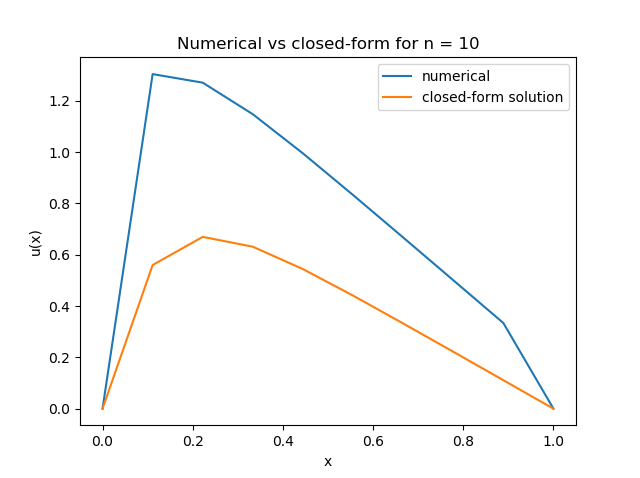
\includegraphics[scale = 0.7]{Figures/Figure_1.png}
		\centering
		\caption{The numerical solution vs the closed-form solution for 10 data-points. Here we can see that they deviate massively.}
	\end{figure}

	\begin{figure}[H]
		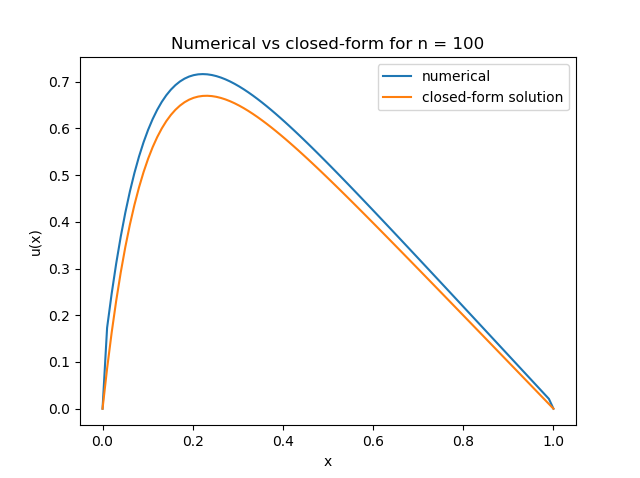
\includegraphics[scale = 0.7]{Figures/Figure_2.png}
		\centering
		\caption{The numerical solution vs the closed-form solution for 100 data-points. Here we can see that the difference is decreasing.}
	\end{figure}

	\begin{figure}[H]
		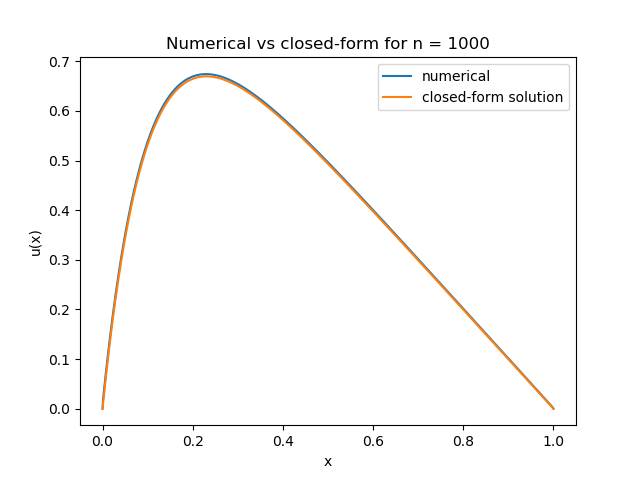
\includegraphics[scale = 0.7]{Figures/Figure_3.png}
		\centering
		\caption{The numerical solution vs the closed-form solution for 100 data-points. Here we can see that the difference has been even more decreased, and it is becoming hard to tell them apart.}
	\end{figure}

	\subsection{Computation time test}
	The general linear equation solver method took $6.4$ seconds to compute $10^6$ data points.\\
	The specific linear equation solver method took $1.0$ seconds to compute $10^6$ data points.

	\subsection{Relative error}
	Using the specific linear equation solver method for data points ranging from $10$ to $10^7$, we got these relative errors:
	\begin{table}[H]
		\begin{tabular}{|c|c|c|c|c|c|c|c|}
		\hline
		n & $10^{1}$ & $10^{2}$ & $10^{3}$ & $10^{4}$ & $10^5$ & $10^6$ & $10^7$\\
		\hline
		$\epsilon_\text{max}$ & $10^{-1}$ & $5.3 \cdot 10^{-3}$ & $4.9 \cdot 10^{-4}$ & $4.8 \cdot 10^{-5}$ & $4.8 \cdot 10^{-6}$ & $4.8 \cdot 10^{-7}$ & $4.8 \cdot 10{-8}$\\
		\hline
		\end{tabular}
	\centering
	\caption{The maximal relative error from the specific linear equation solver. $\epsilon$ is $\log_{10}(|\dfrac{v - u}{u}|)$ where $v$ is the calculated value and $u$ is the closed-form solution.}
	\end{table}
	
	\subsection{Our method vs numpy.linalg.solve}
	Solving the linear equation systems using numpy.linalg.solve and our method for different amounts of data points results in:
	\begin{figure}[H]
		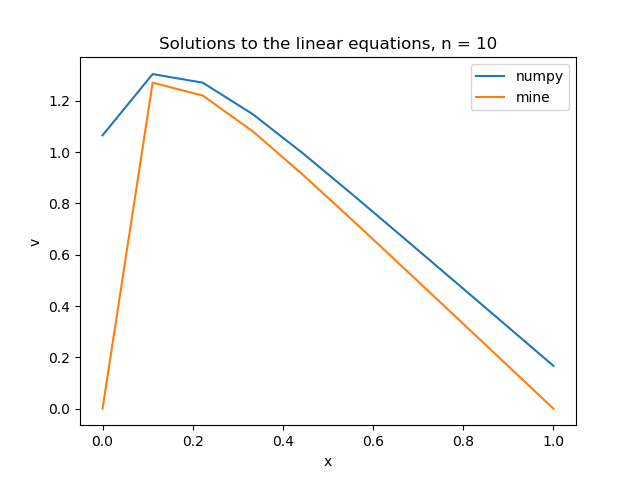
\includegraphics[scale = 0.7]{Figures/Figure_4.png}
		\centering
		\caption{Numpy solution vs my solution. They already seem similair.}
	\end{figure}
	
	\begin{figure}[H]
		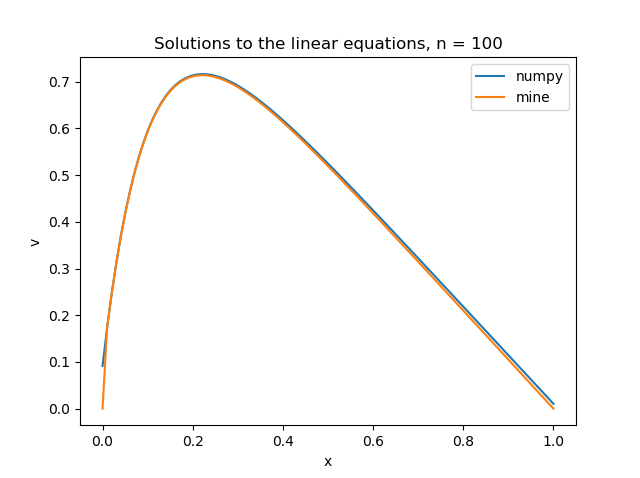
\includegraphics[scale = 0.7]{Figures/Figure_5.png}
		\centering
		\caption{Numpy solution vs my solution. It is becoming harder to tell them apart.}
	\end{figure}

	\begin{figure}[H]
		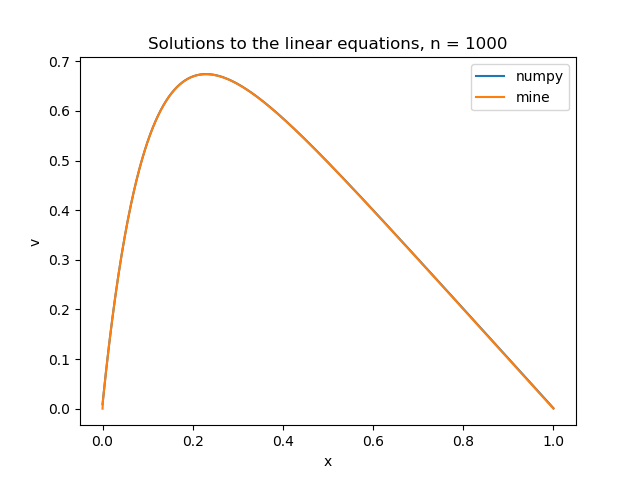
\includegraphics[scale = 0.7]{Figures/Figure_6.png}
		\centering
		\caption{Numpy solution vs my solution. It is now impossible to tell them apart.}
	\end{figure}
	The elapsed time was:
	\begin{table}[H]
		\begin{tabular}{|c|c|c|}
		\hline
		Method & $n = 100$ & $n = 1000$\\
		\hline
		numpy & $0.001$ s & $0.015$ s\\
		\hline
		mine & $0.00097$ s & $0.010$ s\\
		\hline
		\end{tabular}
	\centering
	\caption{Computation time for the 2 methods.}
	\end{table}
\section{Discussion}
	\subsection{Row reduction methods.}
	The easiest, and least efficient, way to implement row reduction seems to be operating directly on a whole matrix using matrix notation. For this project, that was definitely not viable as we did not have enough memory for matrices larger than $10^4 \times 10^4$.\\
	Removing all the zeros and operating on a $n \times 4$ matrix was also quite simple, and required a lot less computation time and memory. It is a shame work was not started on that immediately, as the memory problem was not realised until using $10^5 \times 10^5$ matrices was attempted and the first implementation took some time.\\
	\\
	Making the specified linear equation solver was by far the biggest task this project. The immediate reaction was to find a way to omit any calculations that did not directly apply to $\vec{f}$. The implementation of this eluded success for quite a while, however. This resulted in the implementation of the method "slow\_specific\_linear\_equation\_solver", which follows the same principle as the method "linear\_equation\_solver". Later, implementation of the original idea was attempted once again, and succeded.\\
	The method "fast\_specific\_linear\_equation\_solver" seems to be around 5 times faster than the general one. This seems inconsistent with our calculation of FLOPS. This might be because we counted division to be 1 FLOP, while it is actually more costly than that.

	\subsection{Relative Error}
	From Table 1, it looks like solving the differential equation using row reduction is a first order method, causing the error to be reduced by a factor of 10 when the amount of data-points is increased by a factor of 10.

	\subsection{LU decomposition}
	We can see that the time elapsed inceases faster for the numpy method than for our method. This is no surprise, as the numpy method operates on the whole matrix. The numpy method assumedly has $\frac{2}{3}n^3$ FLOPS. It is impossible to use it on a matrix as large as $10^5 \times 10^5$ as our computer lacks the memory.

\section{Conclusion}
	From these experiments, we see the importance of making less generalized code when operating on very large matrices, as this can cut down on both memory usage and computation time. 

\newpage
\section{Appendix}
	This is the code used in the project.
\lstinputlisting{Code/Fys4150_project1.py}
\end{document}